\chapter{方法}
\label{c:3}

%==========================================================================================
\section{解析YOLO黑盒子}

YOLOv2演算法中,有一個黑盒子darknet-19,本論文著重於解析並呈現其內容與過程。

%==========================================================================================
\subsection{Darknet-19表格}

\begin{table}[htbp]
    \centering
    \begin{tabularx}{\textwidth}{| X | X | X | X | X |}
        \hline
        
Layer & Type & Filters & Size/Stride & Output size \\ \hline
0 &  Convolutional & 32   & 3x3/1 & 416x416\\ \hline
1 &  Maxpool       &      & 2x2/2 & 208x208\\ \hline
2 &  Convolutional & 64   & 3x3/1 & 208x208\\ \hline
3 &  Maxpool       &      & 2x2/2 & 104x104\\ \hline
4 &  Convolutional & 128  & 3x3/1 & 104x104\\ \hline
5 &  Convolutional & 64   & 3x3/1 & 104x104\\ \hline
6 &  Convolutional & 128  & 3x3/1 & 104x104\\ \hline
7 &  Maxpool       &      & 2x2/2 & 52x52\\ \hline
8 &  Convolutional & 256  & 3x3/1 & 52x52\\ \hline
9 &  Convolutional & 128  & 1x1/1 & 52x52\\ \hline
10 & Convolutional & 256  & 3x3/1 & 52x52\\ \hline
11 & Maxpool       &      & 2x2/2 & 26x26\\ \hline
12 & Convolutional & 512  & 3x3/1 & 26x26\\ \hline
13 & Convolutional & 256  & 3x3/1 & 26x26\\ \hline
14 & Convolutional & 512  & 3x3/1 & 26x26\\ \hline
15 & Convolutional & 256  & 1x1/1 & 26x26\\ \hline
16 & Convolutional & 512  & 3x3/1 & 26x26\\ \hline
17 & Maxpool       &      & 2x2/2 & 13x13\\ \hline
18 & Convolutional & 1024  &3x3/1 & 13x13\\ \hline
19 & Convolutional & 512  & 1x1/1 & 13x13\\ \hline
20 & Convolutional & 1024 & 3x3/1 & 13x13\\ \hline
21 & Convolutional & 512  & 1x1/1 & 13x13\\ \hline
22 & Convolutional & 1024 & 3x3/1 & 13x13\\ \hline
23 & Convolutional & 1024 & 3x3/1 & 13x13\\ \hline
24 & Convolutional & 1024 & 3x3/1 & 13x13\\ \hline
25 & Route         & 16	  &       &    \\ \hline
26 & Convolutional & 64   & 1x1/1 & 13x13\\ \hline
27 & Reorg	       &      & /2    & 13x13\\ \hline
28 & Route         & 27 24&       & \\ \hline
29 & Convolutional & 1024 & 3x3/1 & 13x13\\ \hline
30 & Convolutional & 425  & 1x1/1 & 13x13\\ \hline
31 & Detection     &      &       & \\ \hline
    \end{tabularx}
\end{table}

%==========================================================================================
\subsubsection{YOLO運作過程}

YOLO 輸入圖片與結果

\begin{figure}[htbp]
\centering
\begin{minipage}[t]{0.48\textwidth}
\centering
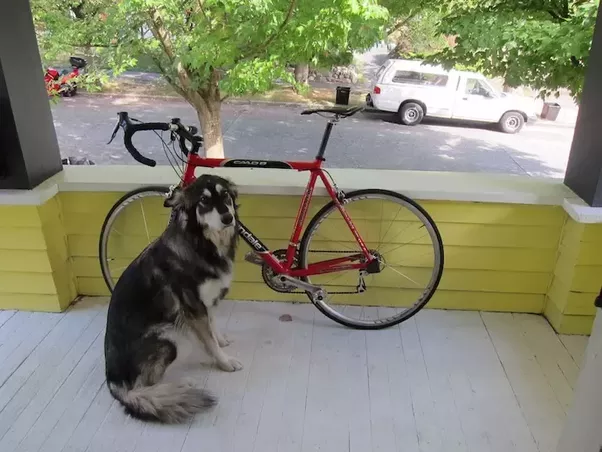
\includegraphics[width=6cm]{fig/ch3_1.png}
\caption{原圖}
\end{minipage}
\begin{minipage}[t]{0.48\textwidth}
\centering
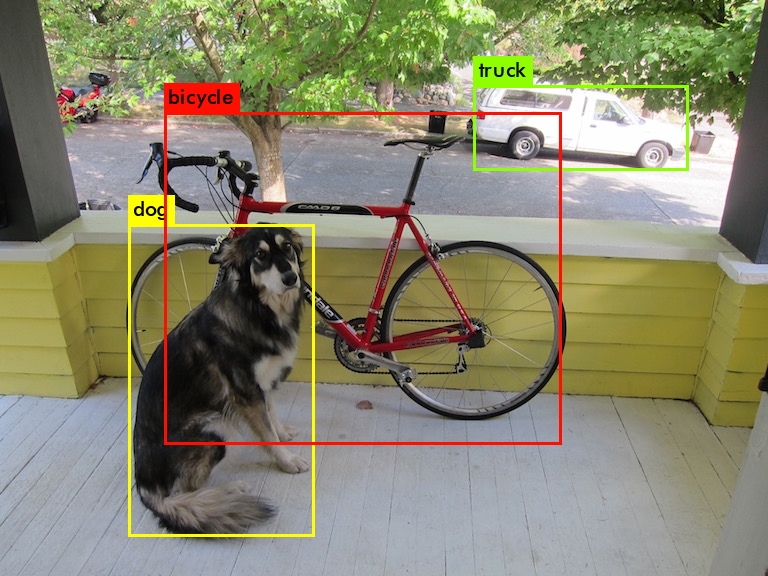
\includegraphics[width=6cm]{fig/ch3_2.png}
\caption{偵測結果}
\end{minipage}
\end{figure}
